%\documentclass[a4paper,11pt]{article}
%\usepackage[a4paper]{}
%\usepackage[utf8]{inputenc}
%\usepackage{listings}
%\usepackage{graphicx}
%\begin{document}

\section{Sensormodulen}
Sensormodulen har som uppgift att läsa in data från robotens sensorer, omvandla dem om det är nödvändigt och vidarebefodra dem till huvudmodulen. För att roboten ska kunna hitta behöver den först veta vart den är och till detta så används två stycken linjesensorer. För att kunna detektera paket kommer roboten på var sin sida ha två avståndssensorer. Om det finns tid så ska det sitta en linjesensor på armen för att kunna detektera formen på paket vilket möjligör utökning till autonom upplockning. Denna kommer förslagsvis bestå av en Atmega16 processor,

\subsection{Reflexsensormodul}
För att kunna beräkna vilken vinkel roboten har i förhållandet till linjen som den följer så har den en reflexmodul fram och en bak. Dessa består av 11 stycken reflexdetektorer som består av en lysdiod och en ljuskänslig transistor. Varje detektor har en enable ingång som slår på ljusdioden och en OUT utgång som ger en analog signal mellan 0V och 5V. Dessa kommer läsas av var för sig och när en detektorer inte läses av kommer enable vara låg för att inte påverka närliggande detektorer samt för att de inte ska överhettas. Avläsningen kommer att ska med två muxar av typen MC14067B vilket är en analog mux med 16 kanaler.

Ett annat förslag är att roboten bara har en reflexsensor längst fram och att den inte reglerar på vinkeln till linjen utan att den reglerar på hur linjen står i förhållande till den främre reflexsensorn.
\subsubsection{Arbetsblock}
\begin{itemize}
\item kalibrera värden
\item ställ in muxarna
\item vänta på lysdiod för att stabilisera sig
\item läs av analog värde
\item omvandla analog värde till digital
\item ta hänsyn till kalibreringen om det är en tejp eller ej under detektorn och trunkera datat efter detta
\item skicka värden till huvudmodulen
\end{itemize}
\subsection{Avståndssensor}
För att kunna detektera om det är ett paket på någon sida av roboten vid stationer så kommer det sitta en avståndssensor på vardera sida av roboten. Dessa kommer vara av typen GP2D120 som är en avståndssensor som använder IR för att generera en analog signal. Denna signal är ej linjär så antingen måste funktionen linjäriseras alternativt så används ett lookuptable som den interpolerar över. Då muxarna som används till reflexsensormodulen har 16 kanaler och de endast använder 11 så kopplas dessa in samma. Dessa kommer dock vara aktiverade hela tiden.
\subsubsection{Arbetsblock}
\begin{itemize}
\item ställ in muxarna
\item läs av analog värde
\item omvandla analog värde till digital
\item kolla upp avstånden i ett lookuptable
\item skicka värden till huvudmodulen
\end{itemize}

\newpage
\subsection{Flödesschema}
Figur \ref{systemskiss:sensorschema} visar flödesschema över mjukvaran i sensormodulen.

%\centerline{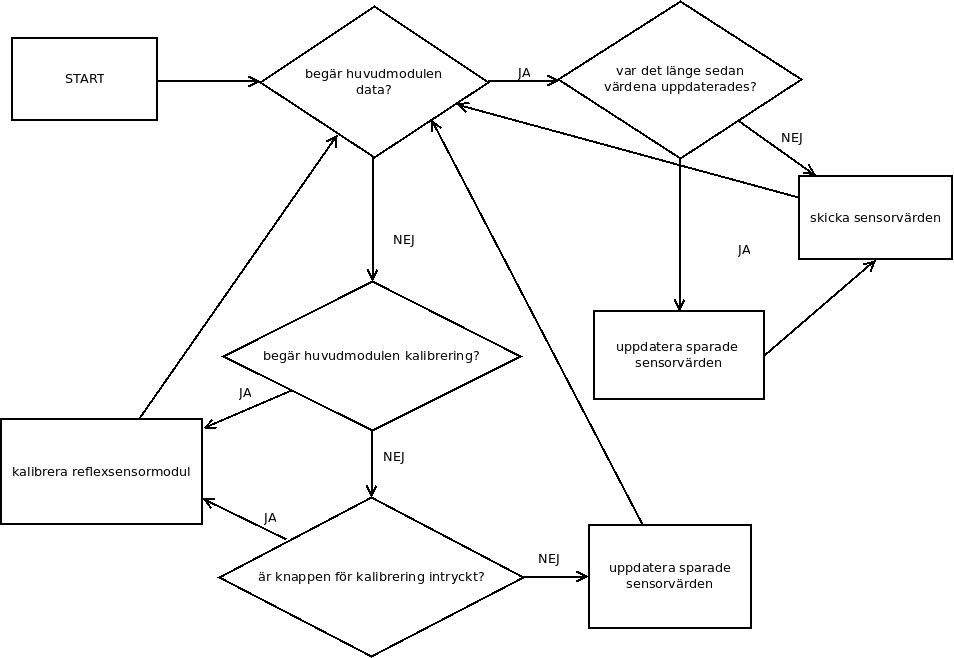
\includegraphics[scale=0.4]{sensorflow}}
%\centerline{Flödesschema för sensormodulen}

\begin{figure}[h]
\center
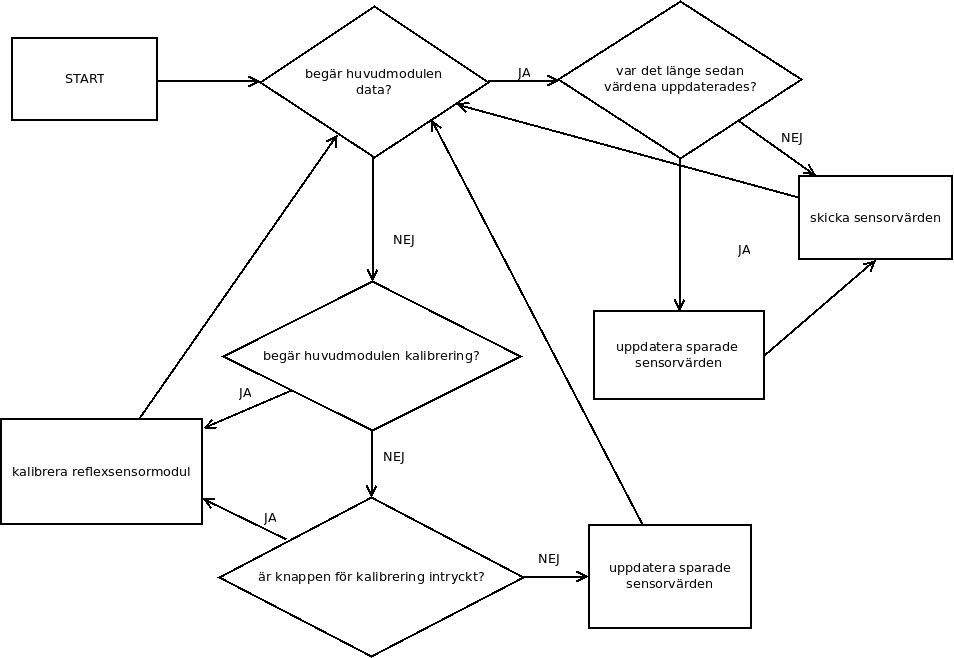
\includegraphics[scale=0.4]{grafik/sensor-flodesschema}
\caption{Flödesschema för sensormodul.} \label{systemskiss:sensorschema}
\end{figure}

%\end{document}
